\documentclass[10pt,twocolumn,letterpaper]{article}

\usepackage{cvpr}
\usepackage{times}
\usepackage{epsfig}
\usepackage{graphicx}
\usepackage{amsmath}
\usepackage{amssymb}
\usepackage{gensymb}

% Include other packages here, before hyperref.

% If you comment hyperref and then uncomment it, you should delete
% egpaper.aux before re-running latex.  (Or just hit 'q' on the first latex
% run, let it finish, and you should be clear).
\usepackage[breaklinks=true,bookmarks=false]{hyperref}

\cvprfinalcopy % *** Uncomment this line for the final submission

\def\cvprPaperID{****} % *** Enter the CVPR Paper ID here
\def\httilde{\mbox{\tt\raisebox{-.5ex}{\symbol{126}}}}

% Pages are numbered in submission mode, and unnumbered in camera-ready
%\ifcvprfinal\pagestyle{empty}\fi
\setcounter{page}{1}
\begin{document}

%%%%%%%%% TITLE
\title{A low-power approach analysis \\ on image-based steering wheel angle prediction models}

\author{
Alessandro Bozzella\\
\texttt{\small Politecnico di Torino}\\
{\tt\small s254764@studenti.polito.it}
\and
Luigi Ferrettino\\
\texttt{\small Politecnico di Torino}\\
{\tt\small s254300@studenti.polito.it}
\and
Rinaldo Clemente\\
\texttt{\small Politecnico di Torino}\\
{\tt\small s259536@studenti.polito.it}
}

\maketitle
%\thispagestyle{}

%%%%%%%%% ABSTRACT
\begin{abstract}
Self-driving vehicles have spread dramatically over the last few years. ADAS control system would have to determine steering wheel angle, brakes and acceleration in any driving environment. The navigation technology in autonomous vehicles is an artificial intelligence application which remains partially unsolved and has been significantly explored by the automotive and technological industries. Many image processing and computer vision techniques allow significant improvements on such recent technologies. In recent years, autonomous driving algorithms, using low-cost vehicle-mounted cameras, have attracted increasing endeavors from both academia and industry. There are multiple fronts to these endeavors, including object detection on roads, 3-D reconstruction etc., but in this work we focus on a cameras-based model that directly maps raw input images to steering angles using deep networks. This represents a nascent research topic in computer vision.
\end{abstract}

%%%%%%%%% BODY TEXT
\section{Introduction}
Nowadays, smart cars are becoming more and more an everyday reality, despite the fact that at this time some autonomous tasks are still really challenging to achieve. The goal of our project is to work around the problem of the steering wheel angle prediction, based \textit{only} on the live images retrieved from the on-board cameras. There are a lot of solutions proposed in the literature, but none of them takes into account the trade-off between accuracy and computational complexity, a climacteric topic when we are talking about the on-board systems, mostly if we are oriented to cheap hardware (for production purposes) that aims at developing accessible cars for everyone. The objective of the proposed approach is basically to solve a regression problem: estimate the steering angle giving a set of images. Therefore, this work uses preexisting CNN architectures as base (PilotNet, LSTM 3D-CONV, ResNet and Transfer Learning) comparing each other on the trade-off between the performance in terms of accuracy and the computational complexity that each model can produce. This analysis showed that the best performing model according to our requirements is the one from Bojarski et al. \cite{Alpher03}. Our goal is to reduce the computational complexity trying not to lose in terms of accuracy. The evaluation will be performed using figures (saliency maps) and plots: the performance metric will be the error on the steering wheel angle prediction with respect to the memory and CPU load. As a final demostration, it has been tested our model on a car simulator game provided by \textit{Udacity}\footnote{\href{https://github.com/udacity/self-driving-car-sim}{\textit{https://github.com/udacity/self-driving-car-sim}}}.

%-------------------------------------------------------------------------
\section{Related Work}
The ambition of autonomous driving can trace back to Leonardo da Vinci's self-propelled cart (if not the earliest), whose complicated control mechanism allows it to follow a pre-programmed path automatically. To date, self-driving cars are no longer a rare sight on real roads. According to Ana Paula G.S. de Almeida et al. \cite{Alpher05}, CNNs are specialized artificial neural networks that process input data with some kind of spatial topology, such as images, videos, audio and text. An artificial neural network is considered convolutional when it has at least one convolution layer and receives a multidimensional input (also referred as a tensor) and applies a series of convolutions using a set of filters. In addition to convolution layers, CNNs are usually composed of other types of layers. Bojarski et al. \cite{Alpher03} have used CNNs (the net is known as PilotNet) to train input camera images to predict the steering wheel angle. They have formulated the steering wheel prediction as a regression problem and have used three cameras (center, left and right) to augment the data set during training, and thus generalize learning. The center camera sees the middle of the road, whereas left and right cameras are tilted sideways. Correction factor is added to the steering angles corresponding to images collected from left and right cameras. Data augmentation techniques such as adding random rotations to the steering angle have also been applied. Deep network architecture uses five convolutional layers followed by five fully-connected layers. As stated by Gaurav Bansal and Dhruv Choudhari \cite{Alpher02}, combination of three-dimensional Convolutional Neural Network (3D-CNN) followed by Long Short-Term Memory (LSTM) model was used to extract the spatio-temporal features. In this form, extraction  of the feature of the image sequences was performed until the end of the 3D-CNN layer, then combine with the last layer before the LSTM layer.

\begin{figure}
    \centering
    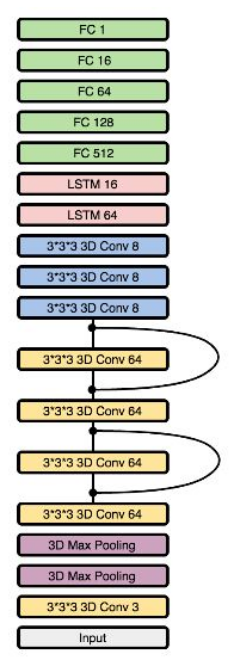
\includegraphics[scale=0.7]{images/image_2020-02-10_18-30-02.png}
    \caption{LSTM 3D-CONV used in \cite{Alpher01}}
    \label{fig:lstm}
\end{figure}

The ResNet model according Lu Chi and Yadong Mu \cite{Alpher04}, first introduced the concept of skip connection. It consists of several different repeating blocks that form residual connections. We still stack convolution layers as before but we now also add the original input to the output of the convolution block. This is referred as \textit{skip connection}. For the work of Andrew Simpson et al. \cite{Alpher01}, transfer learning is a way of using high quality models that were trained on existing large datasets. The idea of transfer learning is that features learned in the lower layers of the model are likely transferable to another dataset. These lower level features would be useful in the new dataset such as edges. In his work, Simpson applied it to an LSTM 3D-CONV architecture (fig.\ref{fig:lstm}). Our work explores several tactics, at multiple stages of the network forwarding procedure. We validate on real data so that the proposed network better captures spatial-temporal information in terms of computational complexity trying to predict the steering wheel angle in the most accurate way.

\section{Dataset and Features}
The dataset used is a merge of the Udacity Dataset 2-2\footnote{\href{http://academictorrents.com/details/bcde779f81adbaae45ef69f9dd07f3e76eab3b27}{\textit{http://academictorrents.com}}} (generated from the NVIDIAs DAVE-2 System \cite{Alpher05}) with a dataset composed only by photos taken from the simulator as if they were real camera mounted on a car. Specifically, data-collecting cars have three cameras mounted at left/middle/right around the rear mirror. Time-stamped video from the cameras is captured simultaneously with the steering angle applied by the human driver. The dataset is made up of a series of images and there is high correlation among adjacent samples, therefore it is important during training to shuffle the training images. Training data was collected by driving on a wide variety of roads and in a different set of lighting and weather conditions and moreover the validation strategy need to be chosen carefully: if we randomize the whole dataset and choose a validation set, we might get very similar images in the validation and training sets. In its entirety, our dataset contains about 300k photos from three different points of view (three cameras).

As a sperimental approach, it has been used the Sobel filter on input images after a greyscale conversion and the other preprocessing stages already explained, in order to extract only the countours of the road. Unfortunately, the results weren't so good.

\subsection{Data Preprocessing and Normalization}
Our preprocessing task starts with the normalization of the value range. Furthermore, images are cropped at the center (66x200x3) to put the sky and trees out of the sight and focus the net on the road. We have used data from left and right cameras to augment the one collected by the center camera; so, as another preprocessing step, we had to adjust the steering angle by a fixed threshold to account the positioning difference between these cameras. These off-center cameras enable training for recovery paths for situations when car might weave from center of the road. Specifically, we adjust the steering angles for images from left and right cameras setting steering correction to a value of 0.2 rad (supposing that the direction of the left and right cams shifts the steering angle of about $\pm 10\degree$) after cross validation.

\subsection{Data Augmentation Methods}
In order to feed the network with every kind of real-world situation, have been applied data augmentation using various random filters.

\begin{figure}[h!]
    \centering
    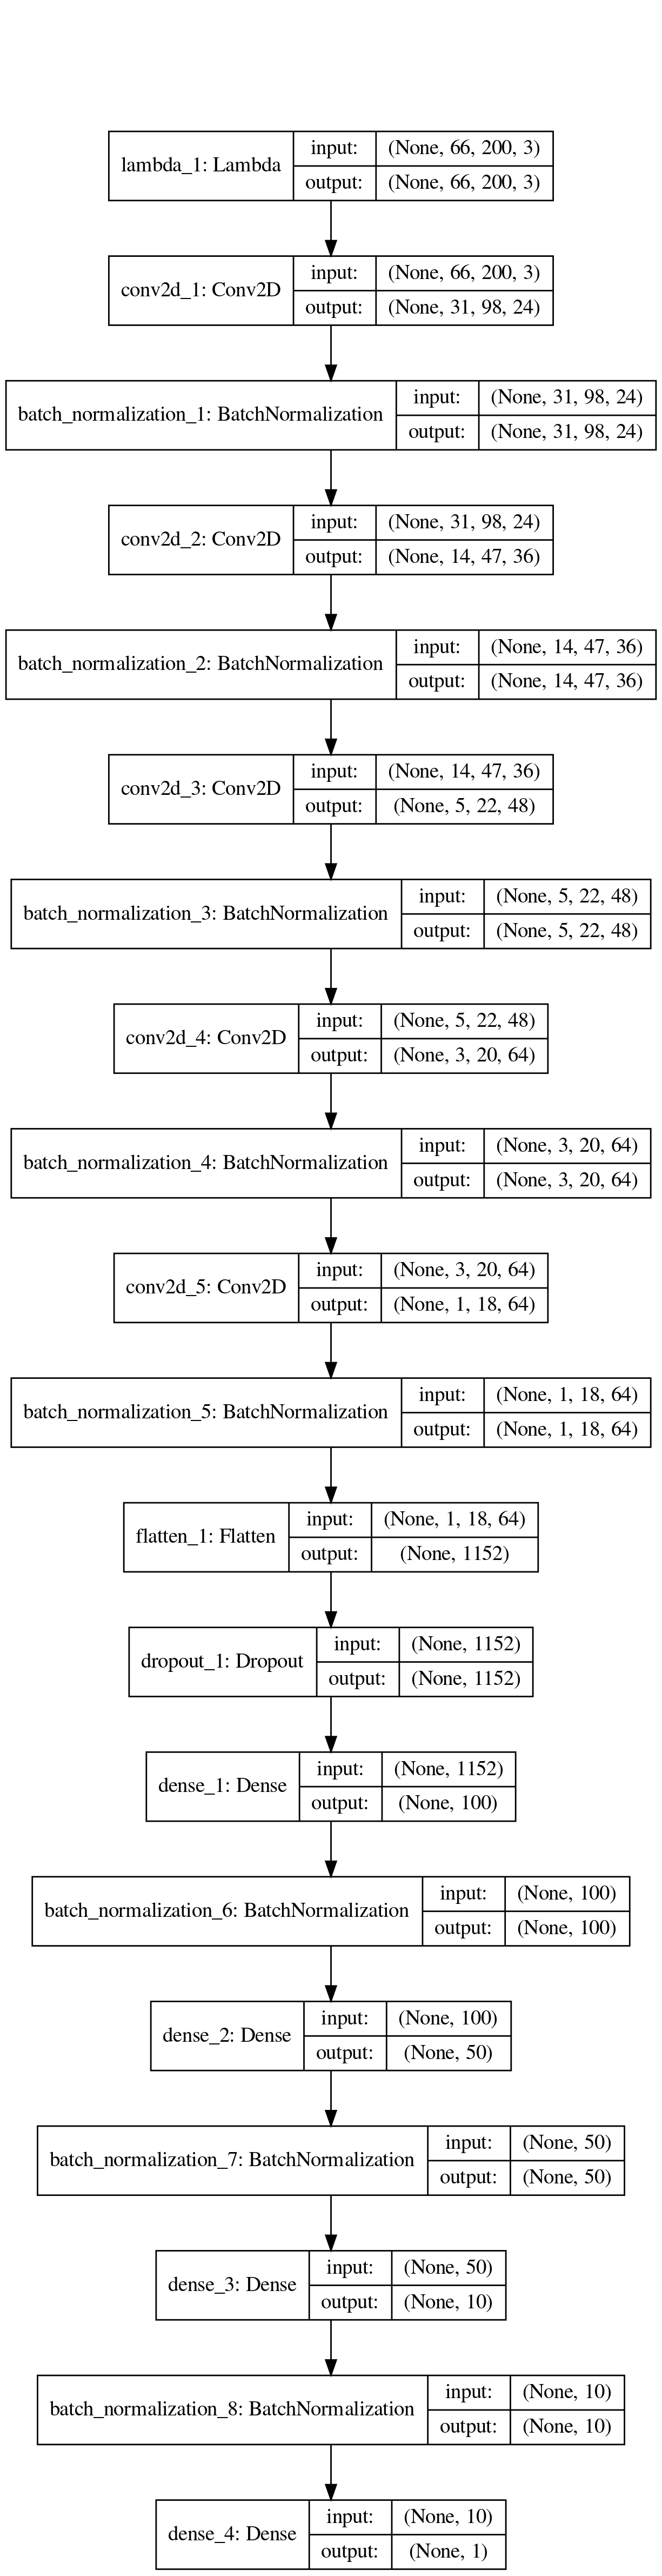
\includegraphics[scale=0.10]{images/model.png}
    \caption{The architecture of the modified NVIDIA PilotNet}
    \label{fig:modell}
\end{figure}

\subsubsection{Random Brightness} 
The brightness of the image can be augmented by either randomly darkening images, brightening images, or both. The intent is to allow a model to generalize across images trained on different lighting levels. This can be achieved by converting images to HSV (Hue Saturation Value), scaling up or down the V channel and converting back to the RGB channel.

\subsubsection{Random Shadow}
From the car's point of view, a shadow is nothing but the dark portions of an image, which could also be bright at times. So a self-driving car is still expected to predict the correct steering angle. This is implemented by choosing random points and shading all points on one side of the image.

\subsubsection{Random Flip}
An image flip reverses the rows or columns of pixels in the case of a vertical or horizontal flip respectively.

\subsubsection{Random Translate}
Translation just involves moving the image along the X or Y direction (or both). This method of augmentation is very useful as most objects can be located almost anywhere in the image. This forces our neural network to look everywhere.

\subsubsection{Random Shift H/V}
A shift to an image means moving all pixels of the image to one direction, such as horizontally or vertically, while keeping the image dimensions the same. We shift the camera images horizontally to simulate the effect of a car in different positions on the road and add an offset corresponding to the shift to the steering angle.

\subsubsection{Others}
Other random filters were applied to simulate snow (single white pixels colouring), fog and rain. In the end, this last technique was not used, because the entire train loop needed more than one day to finish with poor results.

%-------------------------------------------------------------------------
\section{Methods}
The research has been developed in two steps: 

\begin{itemize}
    \item Performance testing and computational complexity derivation of all the models proposed.
    \item General improvement of the best model in terms of computational complexity and validation set error.
\end{itemize}

As regards the first task, three different architectures have been analyzed (both LSTMs and CNNs): the twos from \cite{Alpher01} and the NVIDIA one \cite{Alpher05}. In particular, once they have been trained on the same dataset using the same hyperparameters and same GPU hardware acceleration, they have been validated in order to retrieve the best weights and biases of each one of them. 
Finally, they have been tested on the same test set using the same hardware.

During the testing phase, all the parameters (normalized) of test RMSE (the square root of the MSE) \textit{$t_a$}, RAM consumption \textit{$R_c$}\footnote{The RAM index is normalized on 1GB.} and CPU load \textit{$CPU_l$} were bounded together creating a performance index \textit{$p_i$}. This index is retrieved as follows:

\begin{equation}
    p_i = {RMSE_t}\cdot{R_c}\cdot{CPU_l}
\end{equation}

Using only the CPU (we do not investigate other hardware architecture as GP-GPU, ASIC etc.). The results are written in the table \ref{tab:1}.

As it would be foreseen from the architecture semplicity and a really low number of layers, the NVIDIA PilotNet is the best in terms of performance with respect to the energy consumption\footnote{All the tests have been ran on a i7-8550U machine with DDR4 Dual-Channel RAM without any GPU accaleration.}.

The next step is to add some modifications to it in order to have even better performances.



\begin{table}
\label{tab:1}
\begin{center}
\begin{tabular}{|l|c|c|}
\hline
Method & Test RMSE & Performance index \\
\hline\hline
3D-CONV LSTM & 0.1017 & 5\mathrm{e}{-2} \\
ResNet + TL & 0.0664 & 2.4\mathrm{e}{-2} \\
NVIDIA PilotNet & 0.0931 & \textbf{7.5\mathrm{e}{-3}}\\
\hline
\end{tabular}
\end{center}
\caption{Performance comparison between the models (lower is better).}
\end{table}

In particular, with respect to the original model, it has been also added the Batch Normalization (BN) (on the channel axis for convolutional layers) after each layer for a faster training. It has also been tested using Dropout for regularisation, then fixed at 0.2 after some tests. There has been a lot of debate about when to apply BN, which is either before the non-linearity or after the non-linearity.

\begin{figure}
    \centering
    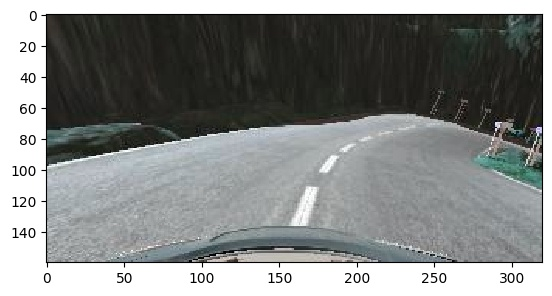
\includegraphics[scale=0.22]{1st-track/no-center_2019_04_02_18_07_15_088.jpg}
    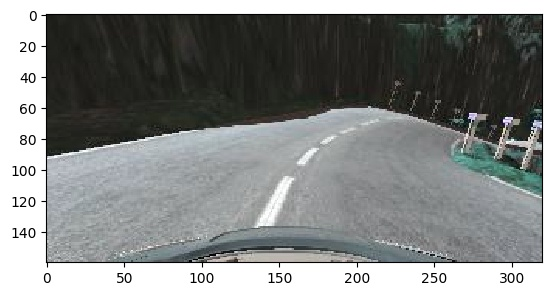
\includegraphics[scale=0.22]{1st-track/no-center_2019_04_02_18_07_15_774.jpg}
    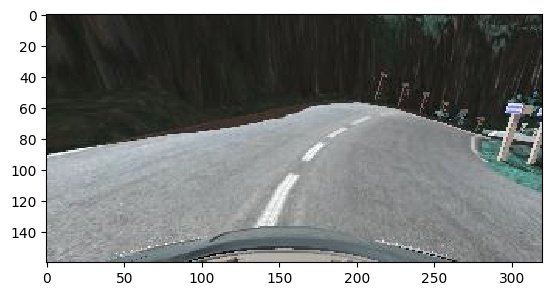
\includegraphics[scale=0.22]{1st-track/no-center_2019_04_02_18_07_16_461.jpg} \\
    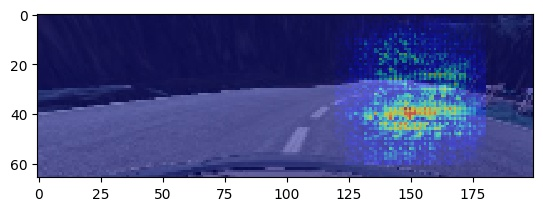
\includegraphics[scale=0.33]{1st-track/yes10-center_2019_04_02_18_07_15_088.jpg} \\
    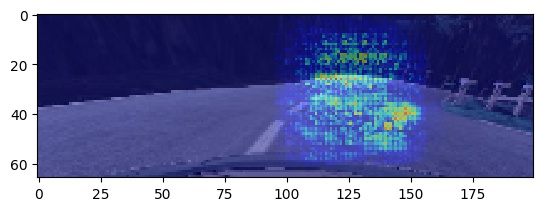
\includegraphics[scale=0.33]{1st-track/yes10-center_2019_04_02_18_07_15_774.jpg} \\
    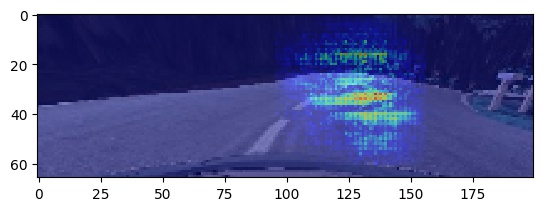
\includegraphics[scale=0.33]{1st-track/yes10-center_2019_04_02_18_07_16_461.jpg} \\
    \caption{Caption}
    \label{fig:track1}
\end{figure}

Since it has been used \textit{ReLu} activation at each layer, applying BN after the ReLu activation was increasing the mean and reducing the variance of the hidden layer activation (BN was not considering the negative activations), hence it has been applied BN after the non-linearity. Following this idea, it has been scaled down the input image to 200x66 (same as PilotNet) in order to keep parameters of the fully connected layers low (the convolutional layers are not affected). This was important to avoid overfitting: models with very high params have a high entropy, leading to overfit (i.e. memorize the training set). With low entropy, gradient descent algorithm forces the model to learn

\begin{figure}[h!]
    \centering
    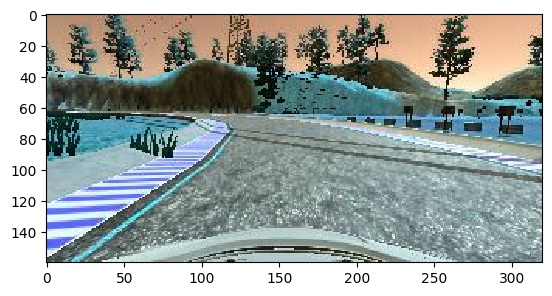
\includegraphics[scale=0.22]{2nd-track/no-center_2019_04_02_19_35_18_729.jpg}
    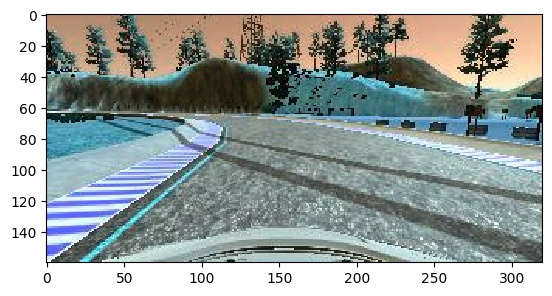
\includegraphics[scale=0.22]{2nd-track/no-center_2019_04_02_19_35_19_438.jpg}
    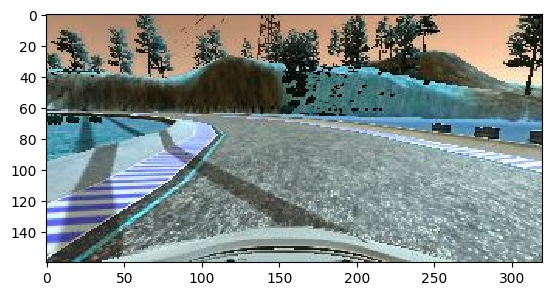
\includegraphics[scale=0.22]{2nd-track/no-center_2019_04_02_19_35_20_131.jpg}
    \\
    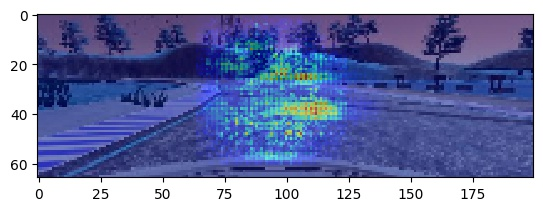
\includegraphics[scale=0.33]{2nd-track/yes10-center_2019_04_02_19_35_18_729.jpg} \\
    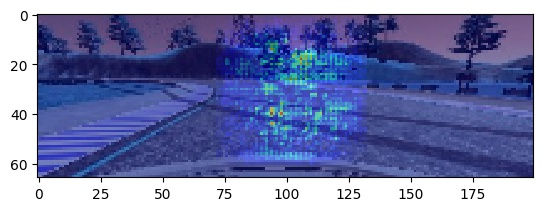
\includegraphics[scale=0.33]{2nd-track/yes10-center_2019_04_02_19_35_19_438.jpg} \\
    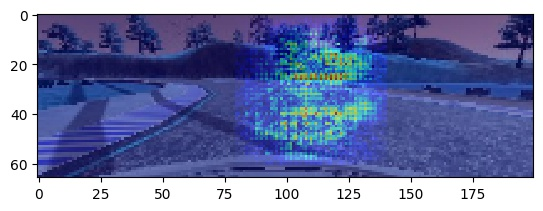
\includegraphics[scale=0.33]{2nd-track/yes10-center_2019_04_02_19_35_20_131.jpg}
    \caption{Caption}
    \label{fig:track2}
\end{figure}

important patterns in the data instead of memorizing the training set. On the other hand, having very low params is also bad as the model may not learn anything. Then, the increase in parameters could have been avoided by using max-pooling, but it is generally used for spatial invariance which is not desired in this case. The input to the model was normalized by dividing the input pixels by 255. There are better ways to normalize input images using the mean and variance of the whole training set but this also works fine. It has been used mean squared error loss without any regularization: these design choices were taken after testing these parameters on the validation set. The rest of the network parameters remain unchanged. The model can be seen in fig. \ref{fig:modell}.





%------------------------------------------------------------------------



\section{Conclusions and Future Work}
The best test set RMSE of the modified model is about 0.0868, a great improvement that takes the performance index to 7e-10.



In order to visualize what the network \textit{see}, three saliency maps have been created  representing the two simulator tracks and the Udacity real dataset by three sequential captures. In capture \ref{fig:track1} the saliency map underlines the intensification of the pixels towards the direction of the future steering angle, permitting a really good estimation in the simulator. In figure \ref{fig:track2} too we can see a similar behaviour, despite the fact that in the second case the car tends firstly to go to the courve boundary and then change the steering.

Finally, a saliency map of a real road is showed in \ref{fig:track3}. It is clear that, while the car is approaching, the network tends to prefer the part of the image where the car must steer (in this case, left).
\vspace{0.5cm}


\begin{figure}[h!]
    \centering
    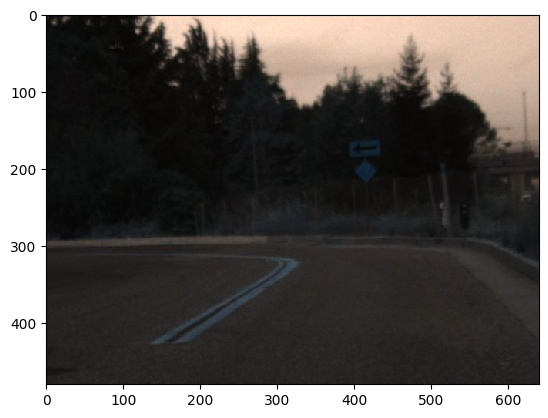
\includegraphics[scale=0.22]{3rd-real/no-1475522434613719763.jpg}
    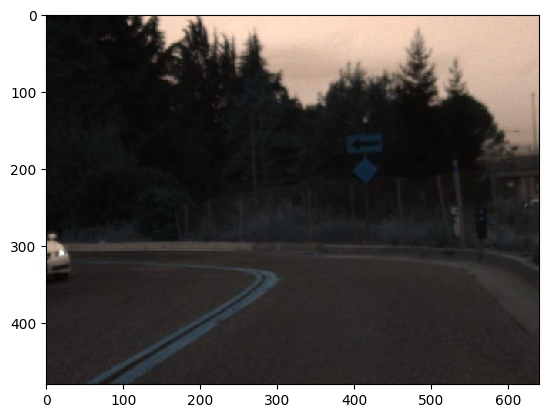
\includegraphics[scale=0.22]{3rd-real/no-1475522435113681487.jpg}
    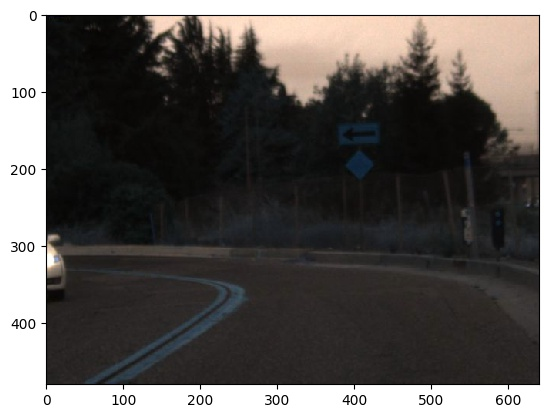
\includegraphics[scale=0.22]{3rd-real/no-1475522435613512147.jpg} \\
    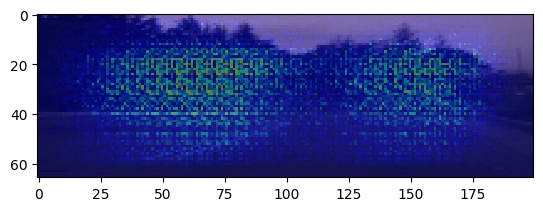
\includegraphics[scale=0.33]{3rd-real/yes10-1475522434613719763.jpg} \\
    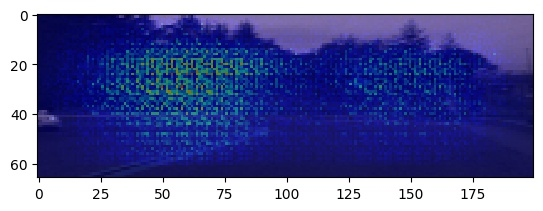
\includegraphics[scale=0.33]{3rd-real/yes10-1475522435113681487.jpg} \\
    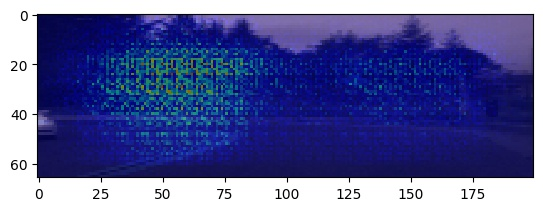
\includegraphics[scale=0.33]{3rd-real/yes10-1475522435613512147.jpg} \\
    \caption{Caption}
    \label{fig:track3}
\end{figure}

One of the problems encountered was the non-uniformity of the merged dataset that leads to poor results shifting the subset from the simulator to the real data. A solution could be a \textit{DANN} architecture from Ganin et al. \cite{Alpher06} in order to exploit domain adaptation. Furthermore, the design of the model could be integrated with V2X technologies that, with the 5G networks that allows low latencies, can reduce the steering error using the live information shared between the cars. It must be pointed out that the weather conditions (created with random modifications) increase the difficulty of the goal, reducing the precision of the prediction and thus the security of the driver. Better analytical approaches are available, such the combination of the Sobel filter \cite{Alpher08} and Hough transform \cite{Alpher09} with the estimation proposed by the Kalman filter \cite{Alpher07}.


Finally, as a demo, it has been added a video record of the proposed model in action, piloting a car on a track in a game.

{\small
\bibliographystyle{ieee_fullname}
\bibliography{egbib}
}

\end{document}
